%!TEX program = xelatex
% 完整编译: xelatex -> biber/bibtex -> xelatex -> xelatex
\documentclass[lang=cn,11pt,a4paper]{elegantpaper}

\usepackage{algorithm}
\usepackage[noend]{algpseudocode}
\usepackage{amsmath}
\usepackage{array}
\usepackage{xcolor}
\usepackage{graphicx}

\lstdefinelanguage{text}{
    showstringspaces=false,
    breaklines=true,
    breakautoindent=true,
    breakindent=0em,
    escapeinside={(*@}{@*)},
    tabsize=4
}

\title{《算法设计与分析》\\课程实验报告}

\author{
\huge 专业:计算机科学与技术 \\[10pt]
\huge 班级:2021211304 \\[10pt]
\huge 姓名:杨晨 \\[10pt]
\huge 学号:2021212171
}
\date{}

% 本文档命令
\usepackage{array}
\newcommand{\ccr}[1]{\makecell{{\color{#1}\rule{1cm}{1cm}}}}

\begin{document}

\maketitle

\clearpage

% \begin{abstract}
% 本文为 \href{https://github.com/ElegantLaTeX/ElegantPaper/}{ElegantPaper} 的说明文档。此模板基于 \LaTeX{} 的 article 类,专为工作论文写作而设计。设计这个模板的初衷是让作者不用关心工作论文的格式,专心写作,从而有更加舒心的写作体验。如果你有其他问题、建议或者报告 bug,可以在 \href{https://github.com/ElegantLaTeX/ElegantPaper/issues}{GitHub::ElegantPaper/issues} 留言。如果你想了解更多 Elegant\LaTeX{} 项目组设计的模板,请访问 \href{https://github.com/ElegantLaTeX/}{GitHub::ElegantLaTeX}。
% \keywords{Elegant\LaTeX{},工作论文,模板}
% \end{abstract}


\section{概述}

\subsection{实验内容}
编程实现下述3个算法, 并利用给定的数据,验证算法正确性,三选一

\begin{enumerate}
    \item 哈夫曼编码
    \begin{itemize}
        \item 针对 “附件2.哈夫曼编码输入文本-23”给出的文本信息,构造哈夫曼编码,文本中的数字0-9、空格、标点符号、控制符参与编码,英文字母区分大小写
        \item 统计26个英文字母、数字0-9、空格、标点符号、控制符的出现的频率
        \item 对{a, b, c,..,x, y, z, 0,…,9, 空格,标点符号},设计哈夫曼编码
        \item 按照哈夫曼编码,对输入文本重新编码
        \item 统计采用哈夫曼编码,输入文本需要的存储比特数,并与定长编码方式需要的存储比特数进行比较
    \end{itemize}
    \item 单源最短路径
    \begin{itemize}
        \item 利用“附件1-1.基站图的邻接矩阵-v1-23”给出的LTE网络基站数据,以基站为顶点,以基站间的距离连线为边,组成图,计算图中的单源最短路径
        \item 图构造
        
        从昆明LTE网络中,选取部分基站,计算基站间的距离,在部分基站间引入边,得到图
        \begin{itemize}
            \item 对22个基站顶点组成的图,以基站567443为源点
             
             计算567443到其它各点的单源最短路径
             
             计算567443到33109的最短路径

            \item 对42个基站顶点组成的图,以基站565845为源点
            
            计算565845到其它各点的单源最短路径
            
            计算565845到565667的最短路径

        \end{itemize}
    \end{itemize}
    \item 最小生成树
    \begin{itemize}
        \item 利用“附件1-1.基站图的邻接矩阵-v1-23”给出的LTE网络基站数据,以基站为顶点,以基站间的距离连线为边,组成图,计算图的最小生成树
        \item 图构造
        
        从昆明LTE网络中,选取部分基站,计算基站间的距离,在部分基站间引入边,得到
        
        22个基站顶点组成的图 
        
        42个基站顶点组成的图
        \item 采用K算法,或P算法,二选一
        \item 给出最小生成树的成本/代价/耗费cost
        \item 做图,展现最小生成树
        
        * 注: 可以在原图上,用红色、粗线条,标记最小生成树
    \end{itemize}
\end{enumerate}

\subsection{开发环境}

\begin{itemize}
    \item Windows10
    \item PyCharm 2023.2.4 (Professional Edition)
    \item Visual Studio Code 1.84.2
\end{itemize}

\section{实验过程}

\subsection{哈夫曼编码}

\subsubsection{介绍}
哈夫曼编码是一种用于数据压缩的算法。它通过对不同字符赋予不同的编码,使得出现频率较高的字符具有较短的编码,从而达到压缩数据的目的。哈夫曼编码的基本思想是根据字符的频率构建一棵二叉树,频率越高的字符离根节点越近,频率越低的字符离根节点越远。在构建的二叉树中,从根节点到叶子节点的路径上的编码表示对应字符。

\subsubsection{算法描述}
下面是使用 C++ 实现的哈夫曼编码算法的伪代码:

\begin{algorithm}[H]
\caption{哈夫曼编码算法}\label{huffman}
\begin{algorithmic}[1]
\Procedure{buildTree}{$freq$}
    \State 创建优先队列$pq$
    \ForAll{$(c, f)$ in $freq$}
        \If{$c$为控制符}
            \State \textbf{continue}
        \EndIf
        \State 创建新的HuffmanNode节点$n$,设置$n$的字符为$c$,频率为$f$,左子节点和右子节点为空
        \State 将$n$插入$pq$
    \EndFor
    \While{$pq$的大小大于$1$}
        \State 从$pq$中取出频率最小的两个节点$left$和$right$
        \State 创建新的HuffmanNode节点$parent$,设置$parent$的字符为空字符,频率为$left$和$right$的频率之和,左子节点为$left$,右子节点为$right$
        \State 将$parent$插入$pq$
    \EndWhile
    \State \textbf{return} $pq$中剩下的唯一节点作为根节点
\EndProcedure

\Procedure{generateCodes}{$root, code, codes$}
    \If{$root$为空}
        \State \textbf{return}
    \EndIf
    \If{$root$的左子节点和右子节点都为空}
        \State 将$code$赋值给$codes[root]$,表示$root$的编码为$code$
        \State \textbf{return}
    \EndIf
    \State 调用\textsc{generateCodes}($root$的左子节点, $code + "0$", $codes$)
    \State 调用\textsc{generateCodes}($root$的右子节点, $code + "1$", $codes$)
\EndProcedure
\end{algorithmic}
\end{algorithm}

\subsubsection{分析}
哈夫曼编码算法的时间复杂度主要集中在两个步骤:构建优先队列$pq$和生成编码字典$codes$。假设输入文本中有$n$个不同的字符。

在构建优先队列的过程中,需要将$n$个节点插入到优先队列中,每次插入的时间复杂度为$O(\log n)$。因此,构建优先队列的时间复杂度为$O(n \log n)$。

在生成编码字典的过程中,对于每个字符,需要在哈夫曼树上进行遍历以找到对应的编码。由于哈夫曼树是一棵二叉树,最坏情况下需要遍历树的高度,即$O(\log n)$。因此,生成编码字典的时间复杂度为$O(n \log n)$。

综上所述,哈夫曼编码算法的总时间复杂度为$O(n \log n)$。

\subsubsection{运行结果}
\begin{lstlisting}[language=text]
字符    频率    哈夫曼编码      定长编码
B       1       1111000010100   000000
P       1       1111000010111   000001
M       1       1111000010101   000010
D       4       11110001110     000011
L       1       001011001000    000100
"       2       101010011000    000101
H       2       001011001001    000110
S       8       1010100101      000111
G       3       00101100111     001000
F       3       00101100110     001001
z       4       11110000010     001010
O       3       00101100101     001011
x       8       1111000100      001100
C       5       11110001111     001101
j       2       111100001000    001110
/       2       111100000111    001111
T       15      101010001       010000
'       2       101010011010    010001
b       103     011110          010010
y       129     101011          010011
1       11      001011000       010100
l       291     11101           010101
g       176     00110           010110
,       55      0111110         010111
f       78      001010          011000
I       7       1010100001      011001
2       2       101010011001    011010
m       243     10100           011011
r       372     0101            011100
4       2       111100001001    011101
o       470     1001            011110
        1078    110             011111
w       77      1111001         100000
a       422     0110            100001
\n      26      00101111        100010
3       2       101010011011    100011
n       317     11111           100100
t       513     1011            100101
W       8       1010100100      100110
-       23      00101101        100111
h       265     11100           101000
i       442     1000            101001
.       66      1010101         101010
s       364     0100            101011
e       677     000             101100
)       8       1111000011      101101
d       158     111101          101110
(       8       1111000000      101111
c       212     01110           110000
5       2       111100000110    110001
p       186     00111           110010
:       6       1010100000      110011
u       167     00100           110100
k       26      00101110        110101
;       1       1111000010110   110110
v       59      0111111         110111
A       9       1111000101      111000
6       8       1010100111      111001
q       9       1111000110      111010
哈夫曼编码存储比特数:31635比特
定长编码存储比特数:42870比特
哈夫曼编码相较定长编码节省空间26.2071%
\end{lstlisting}

\begin{figure}[H]
    \centering
    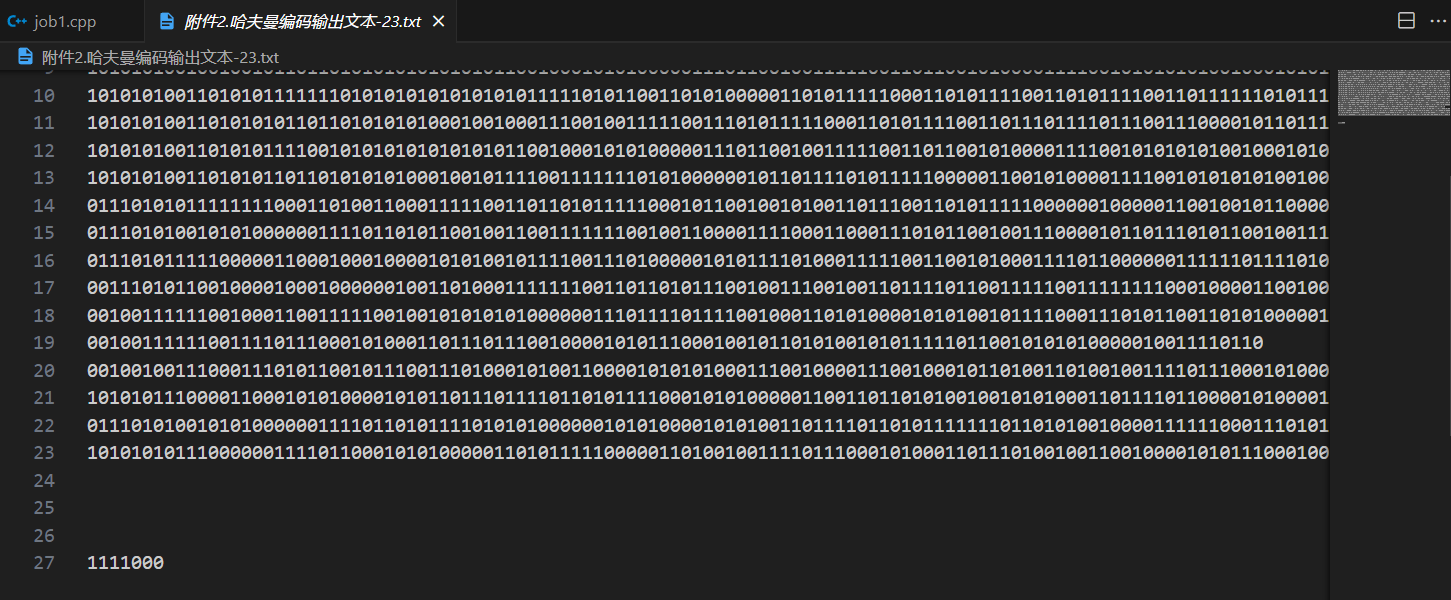
\includegraphics[width=0.9\textwidth]{image/HuffmanEncode.png}
    \caption{哈夫曼编码后的输出文本}
\end{figure}

\subsubsection{结论}
哈夫曼编码是一种有效的数据压缩算法,通过根据字符频率分配不同的编码来实现数据的压缩。该算法的时间复杂度为$O(n \log n)$,其中$n$是不同字符的数量。通过比较哈夫曼编码和定长编码的存储比特数,我们可以看到哈夫曼编码在频率较高的字符上具有更好的压缩效果。因此,哈夫曼编码在数据压缩和存储方面具有广泛的应用前景。


\subsection{单源最短路径}

\subsubsection{介绍}
单源最短路径问题是在给定一个加权有向图中寻找从一个固定起点到所有其他顶点的最短路径的问题。该问题在实际应用中具有广泛的应用,例如路由算法、地图导航等。下面是Dijkstra算法,它是解决单源最短路径问题的经典算法之一。

\subsubsection{算法描述}
Dijkstra算法是一种贪心算法,用于解决单源最短路径问题。它通过逐步确定从起点到每个顶点的最短路径,并将其保存在一个距离数组中。

\begin{algorithm}[H]
\caption{Dijkstra算法}
\begin{algorithmic}[1]
\Procedure{dijkstra}{$adjacency\_matrix$,$start$}
    \State $n \leftarrow$ 邻接矩阵的大小
    \State 初始化$dis$为长度为$n$的数组,初始值为正无穷 \Comment{$dis[i]$表示从$start$到$i$的最短距离}
    \State $dis[start] \leftarrow 0$
    \State 初始化$visited$为长度为$n$的数组,初始值为False
    \For{$i \leftarrow 0$ to $n-1$}
        \State $u \leftarrow -1$
        \State $min\_dis \leftarrow$ 正无穷
        \For{$j \leftarrow 0$ to $n-1$}
            \If{not $visited[j]$ and $dis[j] < min\_di$}
                \State $u \leftarrow j$
                \State $min\_di \leftarrow dis[j]$
            \EndIf
        \EndFor
            \If{$u = -1$}
                \State \textbf{break}
            \EndIf
            \State $visited[u] \leftarrow$ True
        \For{$v \leftarrow 0$ to $n-1$}
            \If{$adjacency\_matrix[u][v] = -1$}
                \State \textbf{continue}
            \EndIf
            \If{not $visited[v]$ and $dis[v] > dis[u] + adjacency\_matrix[u][v]$}
                \State $dis[v] \leftarrow dis[u] + adjacency\_matrix[u][v]$
            \EndIf
        \EndFor
    \EndFor
    \If{$len(visited) != n$}
        \State $print$ 不连通
        \State \Return $None$
    \EndIf
    \State \Return $dis$
\EndProcedure
\end{algorithmic}
\end{algorithm}

\subsubsection{分析和改进}
原始的Dijkstra算法的时间复杂度为$O(V^2)$,其中$V$是顶点的数量。然而,通过使用优先队列(例如堆)来维护候选顶点集合,我们可以改进算法的时间复杂度。

以下是改进后的Dijkstra算法的伪代码:

\begin{algorithm}[H]
\caption{改进后的Dijkstra算法}
\begin{algorithmic}[1]
\Procedure{dijkstra\_saving\_time}{$adjacency\_matrix$,$start$}
    \State 初始化$dis$为长度为$n$的数组,初始值为正无穷
    \State $dis[start] \leftarrow 0$
    \State 初始化$visited$为长度为$n$的数组,初始值为False
    \State 初始化空的优先队列$heap$
    \State 将$(0.0, start)$插入$heap$
    \While{$heap$不为空}
        \State $(d, u) \leftarrow$ 从$heap$中弹出最小元素
        \If{$visited[u]$}
            \State \textbf{continue}
        \EndIf
        \State $visited[u] \leftarrow$ True
        \For{$v \leftarrow 0$ to $n-1$}
            \If{$adjacency\_matrix[u][v] = -1$}
                \State \textbf{continue}
            \EndIf
            \If{not $visited[v]$ and $dis[v] > dis[u] + adjacency\_matrix[u][v]$}
                \State $dis[v] \leftarrow dis[u] + adjacency\_matrix[u][v]$
                \State 将$(dis[v], v)$插入$heap$
            \EndIf
        \EndFor
    \EndWhile
    \If{$len(visited) != n$}
        \State $print$ 不连通
        \State \Return $None$
    \EndIf
    \State \Return $dis$
\EndProcedure
\end{algorithmic}
\end{algorithm}

改进后的Dijkstra算法的时间复杂度为$O((V+E)\log V)$,其中$V$是顶点的数量,$E$是边的数量。通过使用优先队列来选择下一个最短路径顶点,我们减少了在每次迭代中查找最小距离顶点的时间。
\subsubsection{运行结果}
\begin{lstlisting}[language=text]
(*@\textcolor{orange}{以567443为起点,到各点的最短距离为}@*)
33109: 1956.93
565696: 1343.41
566631: 761.94
566720: 2111.29
566742: 302.54
566747: 1988.14
566750: 683.09
566751: 1622.91
566783: 344.55
566798: 1778.06
566802: 963.85
566967: 1562.25
566993: 988.63
566999: 2072.92
567203: 1592.31
567238: 780.89
567260: 244.05
567322: 1582.91
567439: 1309.05
567443: 0.00
567547: 1733.00
568098: 810.56
(*@\textcolor{green!60!black}{以567443为起点,到33109的最短距离为:1956.93}@*)
(*@\textcolor{green!60!black}{经验证, 优化后的dijkstra算法正确}@*)

(*@\textcolor{orange}{以565845为起点,到各点的最短距离为}@*)
565675: 1369.37
565621: 1928.90
565667: 2900.12
567510: 645.04
565801: 1153.11
566010: 403.43
567891: 2401.90
565492: 2223.01
565558: 2171.29
565627: 2697.46
565572: 2440.92
565610: 2025.89
565859: 2050.98
565630: 1468.96
565559: 2381.34
565845: 0.00
565527: 2594.34
565633: 2347.84
565496: 2308.24
565865: 2489.07
565773: 2281.46
567531: 1402.79
565516: 1918.10
565393: 2339.03
565753: 1122.45
33566: 2169.68
566074: 1573.64
565648: 1997.17
567526: 488.24
565551: 1806.75
565631: 843.92
565608: 1883.38
567500: 1055.67
565531: 2161.48
565562: 853.57
32788: 2187.66
567497: 1561.46
566316: 2592.69
568056: 2787.20
565964: 741.61
567618: 1655.16
565898: 978.43
(*@\textcolor{green!60!black}{以565845为起点,到565667的最短距离为:2900.12}@*)
(*@\textcolor{green!60!black}{经验证, 优化后的dijkstra算法正确}@*)
\end{lstlisting}


\subsubsection{结论}
上面介绍了单源最短路径问题及其解决方案,介绍了Dijkstra算法的原始版本和改进版本,并分析了它们的时间复杂度。通过使用优先队列,改进后的Dijkstra算法能够更高效地找到最短路径。在实际应用中,Dijkstra算法被广泛应用于解决单源最短路径问题。

\subsection{最小生成树}
\subsubsection{介绍}
最小生成树是图论中的一个重要概念,用于找到一个连通图的最小权重生成树。最小生成树在很多应用中都有广泛的应用,例如网络设计、电路设计、城市规划等。下面将介绍两种常用的最小生成树算法:Kruskal 算法和 Prim 算法。

\subsubsection{算法描述}
Kruskal 算法是一种基于边的贪心算法,用于构建最小生成树。它的基本思想是从图的边集中选择具有最小权重的边,然后逐步扩展生成树,直到生成树包含了所有的顶点。下面是 Kruskal 算法的伪代码描述:

\begin{algorithm}[H]
\caption{Kruskal算法}
\begin{algorithmic}[1]
    \Function{Kruskal}{$\text{adjacency\_matrix}$}
        \Comment{最小生成树,Kruskal算法,时间复杂度$O(E\log E)$}
        \Function{find}{$\text{parent}, i$}
            \Comment{查找节点i的根节点}
            \While{$\text{parent}[i] \neq i$}
                \State $i \gets \text{parent}[i]$
            \EndWhile
            \State \textbf{return} $i$
        \EndFunction
        
        \Procedure{union}{$\text{parent}, i, j$}
            \Comment{合并i和j所在的集合}
            \State $i_{\text{root}} \gets \text{find}(\text{parent}, i)$
            \State $j_{\text{root}} \gets \text{find}(\text{parent}, j)$
            \If{$i_{\text{root}} \neq j_{\text{root}}$}
                \State $\text{parent}[i_{\text{root}}] \gets j_{\text{root}}$
            \EndIf
        \EndProcedure
        
        \State $n \gets \text{len}(\text{adjacency\_matrix})$
        \State $\text{edges\_list} \gets []$
        
        \For{$i \gets 0$ \textbf{到} $n-1$}
            \For{$j \gets 0$ \textbf{到} $n-1$}
                \If{$\text{adjacency\_matrix}[i][j] \neq -1$}
                    \State $\text{edges\_list.append}((i, j, \text{adjacency\_matrix}[i][j]))$
                \EndIf
            \EndFor
        \EndFor
        
        \State $\text{edges\_list.sort(key}=\lambda x: x[2])$
        \State $\text{edges} \gets []$
        \State $\text{min\_cost} \gets 0$
        \State $\text{parent} \gets [i \text{ for } i \text{ in range}(n)]$
        
        \For{$u, v, \text{cost} \text{ in } \text{edges\_list}$}
            \If{$\text{find}(\text{parent}, u) \neq \text{find}(\text{parent}, v)$}
                \State \text{union}(\text{parent}, u, v)
                \State $\text{min\_cost} \gets \text{min\_cost} + \text{cost}$
                \State $\text{edges.append}((u, v))$
            \EndIf
            
            \If{$\text{len}(\text{edges}) = n - 1$}
                \State \textbf{break}
            \EndIf
        \EndFor
        
        \If{$\text{len}(\text{edges}) \neq n - 1$}
            \State \textbf{print}('不连通')
            \State \textbf{return} \textbf{None}
        \EndIf
        
        \State \textbf{return} $\text{min\_cost}, \text{edges}$
    \EndFunction
\end{algorithmic}
\end{algorithm}


Prim 算法是一种基于顶点的贪心算法,用于构建最小生成树。它的基本思想是从一个顶点开始,逐步选择与当前生成树连接的具有最小权重的边所连接的顶点,直到生成树包含了所有的顶点。下面是 Prim 算法的伪代码描述:

\begin{algorithm}[H]
\caption{Prim算法}
\begin{algorithmic}[1]
    \Function{Prim}{$\text{adjacency\_matrix}$}
        \Comment{最小生成树,Prim算法,时间复杂度$O(n^2)$}
        \State \textbf{Input}: 邻接矩阵 $\text{adjacency\_matrix}$
        \State \textbf{Output}: 最小生成树的权值
        
        \State $n \gets \text{len}(\text{adjacency\_matrix})$
        \State $\text{min\_cost} \gets 0$
        \State $\text{lowcost} \gets [\infty] * n$
        \State $\text{lowcost}[0] \gets 0$
        \State $\text{visited} \gets [\text{False}] * n$
        \State $\text{edges} \gets []$ \Comment{最小生成树的边}
        
        \For{$\text{\_} \gets 0$ \textbf{to} $n-1$}
            \State $\text{min\_dis} \gets \infty$
            \State $u \gets -1$
            
            \For{$i \text{ in range}(n)$}
                \If{not $\text{visited}[i]$ \textbf{and} $\text{lowcost}[i] < \text{min\_dis}$}
                    \State $\text{min\_dis} \gets \text{lowcost}[i]$
                    \State $u \gets i$
                \EndIf
            \EndFor
            
            \If{$u = -1$}
                \State \textbf{break}
            \EndIf
            
            \State $pre\_u \gets \text{next}(pre\_u \text{ for } pre\_u \text{ in range}(n) \text{ if } \text{adjacency\_matrix}[pre\_u][u] = \text{min\_dis})$
            \State $\text{edges.append}((pre\_u, u))$
            \State $\text{min\_cost} \gets \text{min\_cost} + \text{min\_dis}$
            \State $\text{visited}[u] \gets \text{True}$
            
            \For{$v \text{ in range}(n)$}
                \If{$\text{adjacency\_matrix}[u][v] = -1$}
                    \State \textbf{continue}
                \EndIf
                
                \If{not $\text{visited}[v]$ \textbf{and} $\text{adjacency\_matrix}[u][v] < \text{lowcost}[v]$}
                    \State $\text{lowcost}[v] \gets \text{adjacency\_matrix}[u][v]$
                \EndIf
            \EndFor
        \EndFor
        
        \If{$\text{len}(\text{visited}) \neq n$}
            \State \textbf{print}('不连通')
            \State \textbf{return} \textbf{None}
        \EndIf
        
        \State \textbf{return} $\text{min\_cost}, \text{edges}$
    \EndFunction
\end{algorithmic}
\end{algorithm}


\subsubsection{分析和改进}
Kruskal 算法的时间复杂度为 $O(E \log E)$,其中 $E$ 是边的数量。算法首先对边的集合进行排序,时间复杂度为 $O(E \log E)$;然后通过并查集的操作判断边是否形成环路,并将不形成环路的边添加到最小生成树中,时间复杂度为 $O(E \alpha(V))$,其中 $\alpha(V)$ 是 Ackermann 函数的反函数,近似于 $O(\log V)$。综合考虑,Kruskal算法使用并查集后的时间复杂度可以近似看作$O(E \log E + \alpha(V))$。由于通常$E$远小于$V^2$,因此可以进一步简化为O(ElogV)。


Prim算法的时间复杂度为$O(n^2)$,其中$n$是图中顶点的数量。算法的时间复杂度主要来自于每次找到未访问顶点中的最小lowcost值的操作,需要遍历$n$个顶点,每次遍历需要$O(n)$的时间。同时,更新最小距离、标记顶点访问状态以及添加边的操作都可以在常数时间内完成。

然而,如果图是稀疏的,即顶点数$n$远大于边数$E$,可以考虑使用优先队列(例如最小堆)来维护未访问顶点中的最小lowcost值,从而将时间复杂度降低,这样可以更快地找到最小值。伪代码如下:

\begin{algorithm}[H]
\caption{堆优化Prim算法}
\begin{algorithmic}[1]
\Function{Prim}{$\text{adjacency\_matrix}$}
    \State $n \gets \text{len}(\text{adjacency\_matrix})$
    \State $\text{min\_cost} \gets 0$
    \State $\text{lowcost} \gets [\infty] * n$
    \State $\text{lowcost}[0] \gets 0$
    \State $\text{visited} \gets [\text{False}] * n$
    \State $\text{heap} \gets [(0.0, 0)]$  \Comment{(权值, 下标)}
    \State $\text{edges} \gets []$  \Comment{最小生成树的边}
    \While{$\text{heap}$ is not empty}
        \State $(\text{cost}, u) \gets \text{heappop}(\text{heap})$
        \If{$\text{visited}[u]$}
            \State \textbf{continue}
        \EndIf
        \State $\text{min\_cost} \gets \text{min\_cost} + \text{cost}$
        \State $\text{visited}[u] \gets \text{True}$
        \State $\text{pre\_u} \gets \text{next}((\text{pre\_u} \text{ for } \text{pre\_u} \text{ in range}(n) \text{ if } \text{adjacency\_matrix}[\text{pre\_u}][u] = \text{cost}), \text{None})$
        \State $\text{edges.append}((\text{pre\_u}, u))$
        \For{$v$ \textbf{in} range($n$)}
            \If{$\text{adjacency\_matrix}[u][v] = -1$}
                \State \textbf{continue}
            \EndIf
            \If{not $\text{visited}[v]$ \textbf{and} $\text{adjacency\_matrix}[u][v] < \text{lowcost}[v]$}
                \State $\text{lowcost}[v] \gets \text{adjacency\_matrix}[u][v]$
                \State $\text{heappush}(\text{heap}, (\text{lowcost}[v], v))$
            \EndIf
        \EndFor
    \EndWhile
    \If{$\text{len}(\text{visited}) \neq n$}
        \State \textbf{print}('不连通')
        \State \textbf{return} \textbf{None}
    \EndIf
    \State \textbf{return} \text{min\_cost}, \text{edges}
\EndFunction
\end{algorithmic}
\end{algorithm}


优化后的Prim 算法的时间复杂度为 $O((V + E) \log V)$,其中 $V$ 是顶点的数量,$E$ 是边的数量。算法使用了优先队列来选择具有最小权重的边,每次从队列中取出具有最小权重的边的时间复杂度为 $O(\log V)$。在每次选择边后,需要更新与新加入的顶点相连的边的权重,并将其插入优先队列中,时间复杂度为 $O(E \log V)$。因此,总的时间复杂度为 $O((V + E) \log V)$。


\subsubsection{运行结果}
\begin{lstlisting}[language=text]
Prim算法最小生成树的权值: 6733.57
Kruskal算法最小生成树的权值: 6733.57
经检验, Prim算法和Prim_saving_time算法结果相同
\end{lstlisting}

\begin{figure}[H]
    \centering
    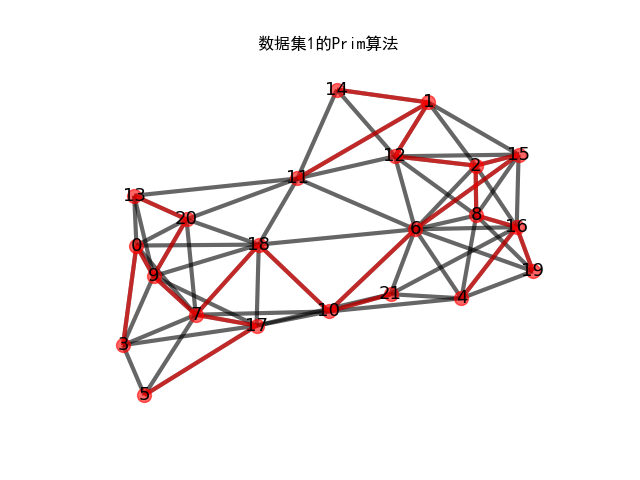
\includegraphics[width=0.9\textwidth, height=0.38\textheight]{image/数据集1的Prim算法.png}
\end{figure}

\begin{figure}[H]
    \centering
    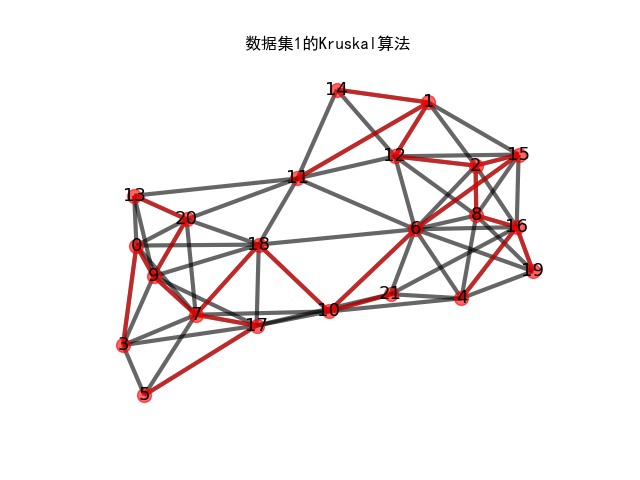
\includegraphics[width=0.9\textwidth, height=0.38\textheight]{image/数据集1的Kruskal算法.png}
\end{figure}

\begin{lstlisting}
Prim算法最小生成树的权值: 13027.03
Kruskal算法最小生成树的权值: 13027.03
经检验, Prim算法和Prim_saving_time算法结果相同
\end{lstlisting}

\begin{figure}[H]
    \centering
    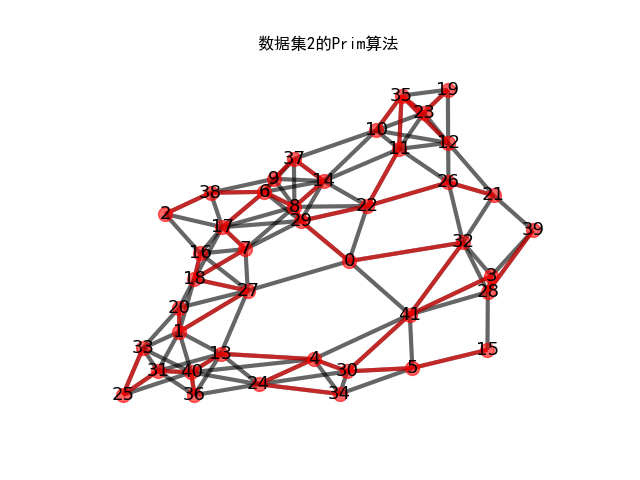
\includegraphics[width=0.9\textwidth, height=0.38\textheight]{image/数据集2的Prim算法.png}
\end{figure}

\begin{figure}[H]
    \centering
    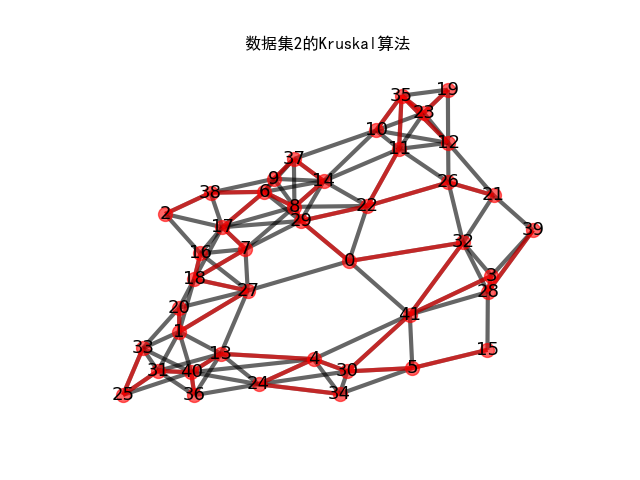
\includegraphics[width=0.9\textwidth, height=0.38\textheight]{image/数据集2的Kruskal算法.png}
\end{figure}

\subsubsection{结论}
综上所述,Prim算法和Kruskal算法都是用于解决最小生成树问题的常见算法。两种算法都可以用于求解最小生成树问题,选择哪种算法取决于具体的应用场景和问题要求。Prim算法在稠密图上的效果较好,而Kruskal算法在稀疏图上的效果较好。

\section{附录:完整代码}

\subsection{哈夫曼编码}
\begin{lstlisting}[language=c++]
#include <iostream>
#include <fstream>
#include <string>
#include <unordered_map>
#include <vector>
#include <queue>
#include <bitset>
#include <iomanip>
#include <cmath>

void input(std::unordered_map<char, int> &freq)
{
    std::ifstream file("附件2.哈夫曼编码输入文本-23.txt");

    if (!file.is_open())
    {
        std::cout << "无法打开文件!" << std::endl;
        return;
    }

    char c;
    while (file.get(c))
    {
        if (freq.find(c) == freq.end())
        {
            freq[c] = 1;
        }
        else
        {
            freq[c]++;
        }
    }

    file.close();
}

class HuffmanNode
{
public:
    char character;
    int frequency;
    HuffmanNode *left;
    HuffmanNode *right;
    // 构造函数
    HuffmanNode(char c, int freq) : character(c), frequency(freq), left(nullptr), right(nullptr) {}
};

struct CompareNodes // 用于优先队列的比较函数, 使得优先队列中的节点按照频率从小到大排列
{
    bool operator()(HuffmanNode *a, HuffmanNode *b)
    {
        return a->frequency > b->frequency;
    }
};

HuffmanNode *buildTree(std::unordered_map<char, int> &freq)
{
    std::priority_queue<HuffmanNode *, std::vector<HuffmanNode *>, CompareNodes> pq;
    for (auto &p : freq)
    {
        pq.push(new HuffmanNode(p.first, p.second));
    }

    while (pq.size() > 1)
    {
        HuffmanNode *left = pq.top();
        pq.pop();
        HuffmanNode *right = pq.top();
        pq.pop();
        HuffmanNode *parent = new HuffmanNode('\0', left->frequency + right->frequency);
        parent->left = left;
        parent->right = right;
        pq.push(parent);
    }

    return pq.top();
}

void generateCodes(HuffmanNode *root, std::string code, std::unordered_map<char, std::string> &codes)
{
    if (root == nullptr)
    {
        return;
    }

    if (root->left == nullptr && root->right == nullptr)
    {
        codes[root->character] = code;
        return;
    }

    generateCodes(root->left, code + "0", codes);
    generateCodes(root->right, code + "1", codes);
}

void printFrequenciesAndCodes(std::unordered_map<char, int> &freq, std::unordered_map<char, std::string> &codes)
{
    int totalBitsHuffman = 0;
    int totalBitsFixed = 0;
    int bitLength = ceil(log2(freq.size())); // 定长编码的二进制数的位数
    int count = 0;                           // 用于计算定长编码的二进制数

    std::cout << std::left << std::setw(8) << "字符" << std::setw(8) << "频率" << std::setw(16) << "哈夫曼编码" << std::setw(16) << "定长编码" << std::endl;
    for (auto &p : freq)
    {
        char character = p.first;
        int frequency = p.second;
        
        std::string huffmanCode = codes[character];
        std::string fixedCode = std::bitset<8>(count++).to_string();
        fixedCode = fixedCode.substr(fixedCode.length() - bitLength, bitLength);

        totalBitsHuffman += frequency * huffmanCode.length();
        totalBitsFixed += frequency * bitLength;

        if (character == '\n') // 换行符
        {
            std::cout << std::left << std::setw(8) << "\\n" << std::setw(8) << frequency << std::setw(16) << huffmanCode << std::setw(16) << fixedCode << std::endl;
            continue;
        }

        std::cout << std::left << std::setw(8) << character << std::setw(8) << frequency << std::setw(16) << huffmanCode << std::setw(16) << fixedCode << std::endl;
    }

    std::cout << "哈夫曼编码存储比特数:" << totalBitsHuffman << "比特" << std::endl;
    std::cout << "定长编码存储比特数:" << totalBitsFixed << "比特" << std::endl;
    std::cout << "哈夫曼编码相较定长编码节省空间" << (1 - (double)totalBitsHuffman / totalBitsFixed) * 100 << "%" << std::endl;
}

void encode(std::unordered_map<char, int> &freq, std::unordered_map<char, std::string> &codes)
{
    std::ifstream file("附件2.哈夫曼编码输入文本-23.txt");

    if (!file.is_open())
    {
        std::cout << "无法打开文件!" << std::endl;
        return;
    }

    std::ofstream fileEncoded("附件2.哈夫曼编码输出文本-23.txt");

    if (!fileEncoded.is_open())
    {
        std::cout << "无法打开文件!" << std::endl;
        return;
    }

    char c;
    while (file.get(c))
    {
        if (c == '\n') // 控制符不参与编码
        {
            fileEncoded << c;
            continue;
        }
        fileEncoded << codes[c];
    }

    file.close();
    fileEncoded.close();
}

int main()
{
    std::unordered_map<char, int> freq;
    input(freq);
    HuffmanNode *root = buildTree(freq);
    std::unordered_map<char, std::string> codes;
    generateCodes(root, "", codes);
    printFrequenciesAndCodes(freq, codes);
    encode(freq, codes);
    return 0;
}

\end{lstlisting}


\subsection{单源最短路径}
\begin{lstlisting}[language=python]
import pandas as pd
import heapq
import numpy as np


def init_data(num):
    """
    初始化数据
    :param num: 数据集编号,[1,2]
    :return: 邻接矩阵, 下标对应的基站id
    """
    df = pd.read_excel('附件1-1.基站图的邻接矩阵-v1-23.xls', sheet_name='数据' + num, header=None)
    size = 0
    if num == '1':
        size = 24
    elif num == '2':
        size = 44
    # 邻接矩阵
    adjacency_matrix = df.values[2:size, 2:size].astype(float)
    # 下标对应的基站id
    station_ids = df.values[2:size, 1].astype(int)
    return adjacency_matrix, station_ids


# 单源最短路径dijkstra算法, 时间复杂度O(V^2)
def dijkstra(adjacency_matrix, start):
    """
    单源最短路径dijkstra算法, 时间复杂度O(V^2)
    :param adjacency_matrix: 邻接矩阵
    :param start: 起点
    :return: dis[i]表示从start到i的最短距离
    """
    n = len(adjacency_matrix)
    # 初始化
    dis = [float('inf')] * n
    dis[start] = 0
    visited = [False] * n

    for i in range(n):
        u = -1
        min_dis = float('inf')
        for j in range(n):
            if not visited[j] and dis[j] < min_dis:
                u = j
                min_dis = dis[j]
        if u == -1:
            break
        visited[u] = True
        for v in range(n):
            if adjacency_matrix[u][v] == -1:
                continue
            if not visited[v] and dis[v] > dis[u] + adjacency_matrix[u][v]:
                dis[v] = dis[u] + adjacency_matrix[u][v]

    if len(visited) != n:
        print('不连通')
        return None

    return dis


# 单源最短路径dijkstra算法, 时间复杂度O((V+E)logV)
def dijkstra_saving_time(adjacency_matrix, start):
    """
    单源最短路径dijkstra算法, 时间复杂度O((V+E)logV)
    :param adjacency_matrix: 邻接矩阵
    :param start: 起点
    :return: dis[i]表示从start到i的最短距离
    """
    n = len(adjacency_matrix)
    # 初始化
    dis = [float('inf')] * n
    dis[start] = 0
    visited = [False] * n

    heap = [(0.0, start)]

    while heap:
        d, u = heapq.heappop(heap)
        if visited[u]:
            continue
        visited[u] = True
        for v in range(n):
            if adjacency_matrix[u][v] == -1:
                continue
            if not visited[v] and dis[v] > dis[u] + adjacency_matrix[u][v]:
                dis[v] = dis[u] + adjacency_matrix[u][v]
                heapq.heappush(heap, (dis[v], v))

    if len(visited) != n:
        print('不连通')
        return None

    return dis


def solve(num, start, end):
    """
    解决问题
    :param num: 数据集编号, [1,2]
    :param start: 起点id
    :param end: 终点id
    """
    adjacency_matrix, station_ids = init_data(num)
    start = np.where(station_ids == start)[0][0]
    end = np.where(station_ids == end)[0][0]
    dist = dijkstra(adjacency_matrix, start)
    print(f'\033[93m以{station_ids[start]}为起点,到各点的最短距离为\033[0m')
    for i in range(len(dist)):
        print(f'{station_ids[i]}: {dist[i]:.2f}')
    print(f'\033[92m以{station_ids[start]}为起点,到{station_ids[end]}的最短距离为:{dist[end]:.2f}\033[0m')
    # 验证优化后的dijkstra算法
    new_dist = dijkstra_saving_time(adjacency_matrix, start)
    if dist == new_dist:
        print('\033[92m经验证, 优化后的dijkstra算法正确\033[0m')
    else:
        print('\033[91m经验证, 优化后的dijkstra算法错误\033[0m')
    print()


if __name__ == '__main__':
    solve('1', 567443, 33109)
    solve('2', 565845, 565667)


\end{lstlisting}

\subsection{最小生成树}
\begin{lstlisting}[language=python]
import pandas as pd
import matplotlib.pyplot as plt
import networkx as nx
import heapq
import matplotlib

matplotlib.rc("font", family="SimHei", weight="bold")  # 解决中文乱码
plt.rcParams["axes.unicode_minus"] = False  # 解决负号无法显示的问题


def init_data(num):
    """
    初始化数据
    :param num: 数据集编号,[1,2]
    :return: 邻接矩阵, 下标对应的基站id
    """
    df = pd.read_excel('附件1-1.基站图的邻接矩阵-v1-23.xls', sheet_name='数据' + num, header=None)
    size = 0
    if num == '1':
        size = 24
    elif num == '2':
        size = 44
    # 邻接矩阵
    adjacency_matrix = df.values[2:size, 2:size].astype(float)
    # 下标对应的基站id
    station_ids = df.values[2:size, 1].astype(int)
    return adjacency_matrix, station_ids


def draw(adjacency_matrix, edges, title):
    """
    绘制最小生成树的图形
    :param adjacency_matrix: 邻接矩阵
    :param edges: 最小生成树的边
    :param title: 图形标题
    """
    G = nx.Graph()
    n = len(adjacency_matrix)

    # 添加顶点
    for i in range(n):
        G.add_node(i)

    min_edge = []

    if edges[0][0] is None:  # 去掉第一个空边(None, 0)
        min_edge = edges[1:]
    else:  # Kruskal算法没有空边
        min_edge = edges

    # 添加边
    for i in range(n):
        for j in range(n):
            if adjacency_matrix[i][j] != -1:
                G.add_edge(i, j, weight=adjacency_matrix[i][j])

    # 绘制图形
    pos = nx.spring_layout(G, seed=1)
    fig, ax = plt.subplots()
    ax.set_title(title)
    nx.draw(G, pos, node_size=100, node_color='red', edge_color='black', width=3.0, alpha=0.6, ax=ax)
    nx.draw_networkx_labels(G, pos, font_size=13, font_color='black', alpha=1.0)

    # 绘制最小生成树的边
    nx.draw_networkx_edges(G, pos, edgelist=min_edge, width=3.0, alpha=0.6, edge_color='red')
    plt.savefig(title + '.png')
    plt.show()

# 最小生成树,Prim算法,O(n^2)
def Prim(adjacency_matrix):
    """
    最小生成树,Prim算法,O(n^2)
    :param adjacency_matrix: 邻接矩阵
    :return: 最小生成树的权值
    """
    n = len(adjacency_matrix)
    min_cost = 0
    # 初始化
    lowcost = [float('inf')] * n
    lowcost[0] = 0
    visited = [False] * n
    edges = []  # 最小生成树的边

    for _ in range(n):
        min_dis = float('inf')
        u = -1
        for i in range(n):
            if not visited[i] and lowcost[i] < min_dis:
                min_dis = lowcost[i]
                u = i
        if u == -1:
            break
        pre_u = next((pre_u for pre_u in range(n) if adjacency_matrix[pre_u][u] == min_dis), None)
        edges.append((pre_u, u))
        min_cost += min_dis
        visited[u] = True
        for v in range(n):
            if adjacency_matrix[u][v] == -1:
                continue
            if not visited[v] and adjacency_matrix[u][v] < lowcost[v]:
                lowcost[v] = adjacency_matrix[u][v]

    if len(visited) != n:
        print('不连通')
        return None

    return min_cost, edges


# 最小生成树,Prim算法,O((V+E)logV)
def Prim_saving_time(adjacency_matrix):
    """
    最小生成树,Prim算法,O((V+E)logV)
    :param adjacency_matrix: 邻接矩阵
    :return: 最小生成树的权值
    """
    n = len(adjacency_matrix)
    min_cost = 0
    # 初始化
    lowcost = [float('inf')] * n
    lowcost[0] = 0
    visited = [False] * n
    heap = [(0.0, 0)]  # (权值, 下标)
    edges = []  # 最小生成树的边

    while heap:
        cost, u = heapq.heappop(heap)
        if visited[u]:
            continue
        min_cost += cost
        visited[u] = True
        pre_u = next((pre_u for pre_u in range(n) if adjacency_matrix[pre_u][u] == cost), None)
        edges.append((pre_u, u))
        for v in range(n):
            if adjacency_matrix[u][v] == -1:
                continue
            if not visited[v] and adjacency_matrix[u][v] < lowcost[v]:
                lowcost[v] = adjacency_matrix[u][v]
                heapq.heappush(heap, (lowcost[v], v))

    if len(visited) != n:
        print('不连通')
        return None

    return min_cost, edges


# 最小生成树,Kruskal算法,O(ElogV)
def Kruskal(adjacency_matrix):
    """
    最小生成树,Kruskal算法,O(ElogE)
    :param adjacency_matrix: 邻接矩阵
    :return: 最小生成树的权值
    """

    def find(parent, i):
        """
        查找i的根节点
        :param parent: parent[i]表示i的父节点
        :param i: 节点i
        :return: i的根节点
        """
        while parent[i] != i:
            i = parent[i]
        return i

    def union(parent, i, j):
        """
        合并i和j所在的集合
        :param parent: parent[i]表示i的父节点
        :param i: 节点i
        :param j: 节点j
        """
        i_root = find(parent, i)
        j_root = find(parent, j)
        if i_root != j_root:
            parent[i_root] = j_root

    n = len(adjacency_matrix)
    edges_list = []
    # 初始化
    for i in range(n):
        for j in range(n):
            if adjacency_matrix[i][j] != -1:
                edges_list.append((i, j, adjacency_matrix[i][j]))
    edges_list.sort(key=lambda x: x[2])
    edges = []  # 最小生成树的边
    min_cost = 0
    parent = [i for i in range(n)]

    for u, v, cost in edges_list:
        if find(parent, u) != find(parent, v):
            union(parent, u, v)
            min_cost += cost
            edges.append((u, v))

        if len(edges) == n - 1:
            break

    if len(edges) != n - 1:
        print('不连通')
        return None

    return min_cost, edges


def solve(num):
    adjacency_matrix, station_ids = init_data(num)
    min_cost, edges = Prim(adjacency_matrix)
    print('Prim算法最小生成树的权值: {:.2f}'.format(min_cost))
    draw(adjacency_matrix, edges, '数据集' + num + '的Prim算法')
    min_cost, edges = Kruskal(adjacency_matrix)
    print('Kruskal算法最小生成树的权值: {:.2f}'.format(min_cost))
    draw(adjacency_matrix, edges, '数据集' + num + '的Kruskal算法')
    min_cost_saving_time, edges = Prim_saving_time(adjacency_matrix)
    if min_cost - min_cost_saving_time < 1e-9:
        print('经检验, Prim算法和Prim_saving_time算法结果相同')
    print()


if __name__ == '__main__':
    solve('1')
    solve('2')

\end{lstlisting}

% 时隔两年,本模板迎来更新,中间发生了很多变化,两个主要变化是参考文献与字体设定,\textbf{使用前请务必仔细阅读本文档}。

% \textbf{文献部分}:我们将 bibtex 的默认文献编译方式改为 biblatex,不过我们也提供了两个后端,\lstinline{bibend=biber} 和 \lstinline{bibend=bibtex}。特别需要注意的是,从 0.10 开始,文献文件改为 \lstinline{reference.bib},与 ElegantBook 保持一致,而参考文献的引文样式等更多格式,请参考后文参考文献部分,更多样式可以参考 biblatex 文档。 

% \textbf{字体部分},我们将 newtxtext 宏包的支持方式改为了字体名称设定方式,设定英文字体为 TeX Gyre Terms/Heros,,英文字体部分,根据编译方式选择不同字体。对于一般用户而言,不太需要关心这部分内容。

% 另外,中文请务必使用 \hologo{XeLaTeX} 编译。

% \subsection{模板介绍}

% 此模板基于 \LaTeX{} 的标准文类 article 设计,所以 article 文类的选项也能传递给本模板,比如 \lstinline{a4paper, 11pt} 等等。

% \begin{lstlisting}
% \documentclass[a4paper,11pt]{elegantpaper}
% \end{lstlisting}

% \textbf{注意}:Elegant\LaTeX{} 系列模板已经全部上传至 \href{https://www.overleaf.com/latex/templates/elegantpaper-template/yzghrqjhmmmr}{Overleaf} 上,用户可以在线使用。另外,为了方便国内用户,模板也已经传至\href{https://gitee.com/ElegantLaTeX/ElegantPaper}{码云}。


% \subsection{全局选项}
% 此模板定义了一个语言选项 \lstinline{lang},可以选择英文模式 \lstinline{lang=en}(默认)或者中文模式 \lstinline{lang=cn}。当选择中文模式时,图表的标题引导词以及参考文献,定理引导词等信息会变成中文。你可以通过下面两种方式来选择语言模式:
% \begin{lstlisting}
% \documentclass[lang=cn]{elegantpaper} % or
% \documentclass{cn}{elegantpaper} 
% \end{lstlisting}

% \textbf{注意:} 英文模式下,由于没有添加中文宏包,无法输入中文。如果需要输入中文,可以通过在导言区引入中文宏包 \lstinline{ctex} 或者加入 \lstinline{xeCJK} 宏包后自行设置字体。 
% \begin{lstlisting}
% \usepackage[UTF8,scheme=plain]{ctex}
% \end{lstlisting}

% \subsection{数学字体选项}

% 本模板定义了一个数学字体选项(\lstinline{math}),可选项有三个:
% \begin{enumerate}
%   \item \lstinline{math=cm}(默认),使用 \LaTeX{} 默认数学字体(推荐,无需声明);
%   \item \lstinline{math=newtx},使用 \lstinline{newtxmath} 设置数学字体(潜在问题比较多)。
%   \item \lstinline{math=mtpro2},使用 \lstinline{mtpro2} 宏包设置数学字体,要求用户已经成功安装此宏包。
% \end{enumerate}

% \subsection{中文字体选项}

% 模板提供中文字体选项 \lstinline{chinesefont},可选项有
% \begin{enumerate}
%   \item \lstinline{ctexfont}:默认选项,使用 \lstinline{ctex} 宏包根据系统自行选择字体,可能存在字体缺失的问题,更多内容参考 \lstinline{ctex} 宏包\href{https://ctan.org/pkg/ctex}{官方文档}\footnote{可以使用命令提示符,输入 \lstinline{texdoc ctex} 调出本地 \lstinline{ctex} 宏包文档}。
%   \item \lstinline{founder}:方正字体选项(\textbf{需要安装方正字体}),后台调用 \lstinline{ctex} 宏包并且使用 \lstinline{fontset=none} 选项,然后设置字体为方正四款免费字体,方正字体下载注意事项见后文,用户只需要安装方正字体即可使用该选项。
%   \item \lstinline{nofont}:后台会调用 \lstinline{ctex} 宏包并且使用 \lstinline{fontset=none} 选项,不设定中文字体,用户可以自行设置中文字体,具体见后文。
% \end{enumerate}

% \subsubsection{方正字体选项}
% 由于使用 \lstinline{ctex} 宏包默认调用系统已有的字体,部分系统字体缺失严重,因此,用户希望能够使用其它字体,我们推荐使用方正字体。方正的{\songti 方正书宋}、{\heiti 方正黑体}、{\kaishu 方正楷体}、{\fangsong 方正仿宋}四款字体均可免费试用,且可用于商业用途。用户可以自行从\href{http://www.foundertype.com/}{方正字体官网}下载此四款字体,在下载的时候请\textbf{务必}注意选择 GBK 字符集,也可以使用 \href{https://www.latexstudio.net/}{\LaTeX{} 工作室}提供的\href{https://pan.baidu.com/s/1BgbQM7LoinY7m8yeP25Y7Q}{方正字体,提取码为:njy9} 进行安装。安装时,{\kaishu Win 10 用户请右键选择为全部用户安装,否则会找不到字体。}

% \begin{figure}[!htb]
% \centering
% 
\includegraphics[width=0.9\textwidth]{founder.png}
% \end{figure}

% \subsubsection{其他中文字体}
% 如果你想完全自定义字体\footnote{这里仍然以方正字体为例。},你可以选择 \lstinline{chinesefont=nofont},然后在导言区设置即可,可以参考下方代码:
% \begin{lstlisting}
% \setCJKmainfont[BoldFont={FZHei-B01},ItalicFont={FZKai-Z03}]{FZShuSong-Z01}
% \setCJKsansfont[BoldFont={FZHei-B01}]{FZKai-Z03}
% \setCJKmonofont[BoldFont={FZHei-B01}]{FZFangSong-Z02}
% \setCJKfamilyfont{zhsong}{FZShuSong-Z01}
% \setCJKfamilyfont{zhhei}{FZHei-B01}
% \setCJKfamilyfont{zhkai}[BoldFont={FZHei-B01}]{FZKai-Z03}
% \setCJKfamilyfont{zhfs}[BoldFont={FZHei-B01}]{FZFangSong-Z02}
% \newcommand*{\songti}{\CJKfamily{zhsong}}
% \newcommand*{\heiti}{\CJKfamily{zhhei}}
% \newcommand*{\kaishu}{\CJKfamily{zhkai}}
% \newcommand*{\fangsong}{\CJKfamily{zhfs}}
% \end{lstlisting}



% \subsection{自定义命令}
% 此模板并没有修改任何默认的 \LaTeX{} 命令或者环境\footnote{目的是保证代码的可复用性,请用户关注内容,不要太在意格式,这才是本工作论文模板的意义。}。另外,我自定义了 4 个命令:
% \begin{enumerate}
%   \item \lstinline{\email}:创建邮箱地址的链接,比如 \email{ddswhu@outlook.com};
%   \item \lstinline{\figref}:用法和 \lstinline{\ref} 类似,但是会在插图的标题前添加 <\textbf{图 n}> ;
%   \item \lstinline{\tabref}:用法和 \lstinline{\ref} 类似,但是会在表格的标题前添加 <\textbf{表 n}>;
%   \item \lstinline{\keywords}:为摘要环境添加关键词。
% \end{enumerate}

% \subsection{参考文献}

% 文献部分,本模板调用了 biblatex 宏包,并提供了 biber(默认) 和 bibtex 两个后端选项,可以使用 \lstinline{bibend} 进行修改:

% \begin{lstlisting}
%   \documentclass[bibtex]{elegantpaper}
%   \documentclass[bibend=bibtex]{elegantpaper}
% \end{lstlisting}

% 关于文献条目(bib item),你可以在谷歌学术,Mendeley,Endnote 中取,然后把它们添加到 \lstinline{reference.bib} 中。在文中引用的时候,引用它们的键值(bib key)即可。

% 为了方便文献样式修改,模板引入了 \lstinline{bibstyle} 和 \lstinline{citestyle} 选项,默认均为数字格式(numeric),参考文献示例:\cite{cn1,en2,en3} 使用了中国一个大型的 P2P 平台(人人贷)的数据来检验男性投资者和女性投资者在投资表现上是否有显著差异。

% 如果需要设置为国标 GB7714-2015,需要使用:
% \begin{lstlisting}
%   \documentclass[citestyle=gb7714-2015, bibstyle=gb7714-2015]{elegantpaper} 
% \end{lstlisting}

% 如果需要添加排序方式,可以在导言区加入
% \begin{lstlisting}
%   \ExecuteBibliographyOptions{sorting=ynt}
% \end{lstlisting}

% 启用国标之后,可以加入 \lstinline{sorting=gb7714-2015}。


% \section{使用 newtx 系列字体}

% 如果需要使用原先版本的 \lstinline{newtx} 系列字体,可以通过显示声明数学字体:

% \begin{lstlisting}
% \documentclass[math=newtx]{elegantpaper}
% \end{lstlisting}

% \subsection{连字符}

% 如果使用 \lstinline{newtx} 系列字体宏包,需要注意下连字符的问题。
% \begin{equation}
%   \int_{R^q} f(x,y) dy.\emph{of\kern0pt f}
% \end{equation}

% \begin{lstlisting}
% \begin{equation}
%   \int_{R^q} f(x,y) dy.\emph{of \kern0pt f}
% \end{equation}
% \end{lstlisting}

% \subsection{宏包冲突}

% 有用户反馈模板在使用 \lstinline{yhmath} 以及 \lstinline{esvect} 等宏包时会报错:
% \begin{lstlisting}
% LaTeX Error:
%    Too many symbol fonts declared.
% \end{lstlisting}

% 原因是在使用 \lstinline{newtxmath} 宏包时,重新定义了数学字体用于大型操作符,达到了 {\heiti 最多 16 个数学字体} 的上限,在调用其他宏包的时候,无法新增数学字体。为了减少调用非常用宏包,在此给出如何调用 \lstinline{yhmath} 以及 \lstinline{esvect} 宏包的方法。

% 请在 \lstinline{elegantpaper.cls} 内搜索 \lstinline{yhmath} 或者 \lstinline{esvect},将你所需要的宏包加载语句\textit{取消注释}即可。


% \section{常见问题 FAQ}

% \begin{enumerate}[label=\arabic*).]
%   \item \textit{如何删除版本信息?}\\
%     导言区不写 \lstinline|\version{x.xx}| 即可。
%   \item \textit{如何删除日期?}\\
%     需要注意的是,与版本 \lstinline{\version} 不同的是,导言区不写或注释 \lstinline{\date} 的话,仍然会打印出当日日期,原因是 \lstinline{\date} 有默认参数。如果不需要日期的话,日期可以留空即可,也即 \lstinline|\date{}|。
%   \item \textit{如何获得中文日期?}\\
%     为了获得中文日期,必须在中文模式下\footnote{英文模式下,由于未加载中文宏包,无法输入中文。},使用 \lstinline|\date{\zhdate{2019/10/11}}|,如果需要当天的汉化日期,可以使用 \lstinline|\date{\zhtoday}|,这两个命令都来源于 \href{https://ctan.org/pkg/zhnumber}{\lstinline{zhnumber}} 宏包。
%   \item \textit{如何添加多个作者?}\\
%     在 \lstinline{\author} 里面使用 \lstinline{\and},作者单位可以用 \lstinline{\\} 换行。
%     \begin{lstlisting}
%     \author{author 1\\ org. 1 \and author 2 \\ org. 2 }
%     \end{lstlisting}
%   \item \textit{如何添加中英文摘要?}\\
%     请参考 \href{https://github.com/ElegantLaTeX/ElegantPaper/issues/5}{GitHub::ElegantPaper/issues/5}
% \end{enumerate}


% \section{致谢}

% 特别感谢 \href{https://github.com/sikouhjw}{sikouhjw} 和 \href{https://github.com/syvshc}{syvshc}  长期以来对于 Github 上 issue 的快速回应,以及各个社区论坛对于 ElegantLaTeX 相关问题的回复。特别感谢 ChinaTeX 以及 \href{http://www.latexstudio.net/}{LaTeX 工作室} 对于本系列模板的大力宣传与推广。

% 如果你喜欢我们的模板,你可以在 Github 上收藏我们的模板。

% \nocite{*}
% \printbibliography[heading=bibintoc, title=\ebibname]

% \appendix
% %\appendixpage
% \addappheadtotoc

\end{document}
